\documentclass [a4paper, 12pt]{article}

\usepackage[utf8]{inputenc}
\usepackage{amssymb}
\usepackage{amsmath}
\usepackage{bm}
\usepackage{epsfig}
\usepackage{graphicx}
\usepackage{times}
\usepackage{float}
\usepackage[usenames,dvipsnames]{color}
\usepackage{caption}
\usepackage{subcaption}
\usepackage{hyperref}
\usepackage{cleveref}
\usepackage[version=4]{mhchem}

\textwidth 16 cm
\textheight 23 cm
\setlength{\oddsidemargin}{0.1 cm}
\setlength{\topmargin}{1 cm}
\setlength{\headheight}{0cm}
\setlength{\headsep}{0cm}
\setlength{\footskip}{0.75cm}
\setlength{\parindent}{0cm}
\setlength{\oddsidemargin}{0.1 cm}
\setlength{\itemsep}{10pt}
\bibliographystyle{gcs}

\DeclareUnicodeCharacter{2212}{-}
\newcommand{\matr}[1]{\bm{#1}}  

\begin{document}
 
\begin{figure}[H]
\begin{center}
  
\includegraphics[scale=0.45]{Figures/GCS-hlrs-fzj-lrz.jpg}\\
\end{center}
\end{figure}

\begin{center}
{\LARGE \bf Project Report} \\

\bigskip
\bigskip
\bigskip
\end{center}
\textbf{Period}\\
\phantom{MM}\textit{01.11.2017-26.04.2018}

\bigskip
\textbf{Project title}\\
\phantom{MM}\textit{KKRnano: Quantum description of skyrmions in chiral B20 magnets}

\bigskip
\textbf{Type of project}\\
\phantom{MM} \textit{new project}

%\bigskip
%\textbf{Project ID}\\
%\phantom{MM} \textit{Please provide in case of a project extension}

\bigskip
\textbf{Principal investigator}\\
\phantom{MM} \textit{ Prof. Dr. Stefan Bl{\"u}gel,
Institute for Advanced Simulation and Peter Gr\"unberg Institut, Forschungszentrum J\"ulich, D-52425 J\"ulich, Germany
}

\bigskip
\textbf{Project contributor(s)}\\

\phantom{MM} \textit{Marcel Bornemann,
Institute for Advanced Simulation and Peter Gr\"unberg Institut, Forschungszentrum J\"ulich, D-52425 J\"ulich, Germany
}

\phantom{MM} \textit{Dr. Sergii Grytsiuk,
Institute for Advanced Simulation and Peter Gr\"unberg Institut, Forschungszentrum J\"ulich, D-52425 J\"ulich, Germany
}

\phantom{MM} \textit{Dr. Roman Kováčik,
Institute for Advanced Simulation and Peter Gr\"unberg Institut, Forschungszentrum J\"ulich, D-52425 J\"ulich, Germany
}


\phantom{MM} \textit{Dr. Rudolf Zeller,
Institute for Advanced Simulation and Peter Gr\"unberg Institut, Forschungszentrum J\"ulich, D-52425 J\"ulich, Germany
}

\phantom{MM} \textit{Dr. Phivos Mavropoulos,
Institute for Advanced Simulation and Peter Gr\"unberg Institut, Forschungszentrum J\"ulich, D-52425 J\"ulich, Germany
}

%\phantom{MM} \textit{Dr. Paul F. Baumeister,
%Institute for Advanced Simulation and J\"ulich Supercomputing Centre, Forschungszentrum J\"ulich, D-52425 J\"ulich, Germany
%}


\newpage

\vfill
\tableofcontents
\vfill

\newpage

\begin{itemize}
	\item subject-specific results
	\item Performance on HazelHen
	\item typical job sizes
	\item Parallelization levels (OMP?)
	\item scaling behaviour \cite{brommel_juqueen_2017}
	\item runtimes
\end{itemize}

\section{Introduction}
We have developed a unique electronic structure code, 
KKRnano \cite{zeller_towards_2008,thiess_massively_2012},
specifically designed for petaFLOP computing. Our method scales linearly
with the number of atoms, so that we canrealize system sizes of up to 
half a million atoms in a unit cell if necessary.
\\
Recently, we implemented a relativistic generalization of our algorithm 
enabling us to calculate complex non-collinear magnetic structures, such as skyrmions,
in real space. Skyrmions are two-dimensional magnetization solitons, i.e. two-dimensional
magnetic structures localized in space, topologically protected by a non-trivial
magnetization texture, which has particle-like properties. 
\\
The focus of our work is on the germanide MnGe that is particularly
interesting among the chiral magnetic B20 compounds, as it exhibits a three-dimensional magnetic structure
that is not yet understood (see preliminary results
\cite{tanigaki_real-space_2015,rybakov_new_2016,bornemann_investigation_2017})

\section{Scientific Results}

\begin{figure}[h]
\centering
\begin{subfigure}[b]{0.49\textwidth}
   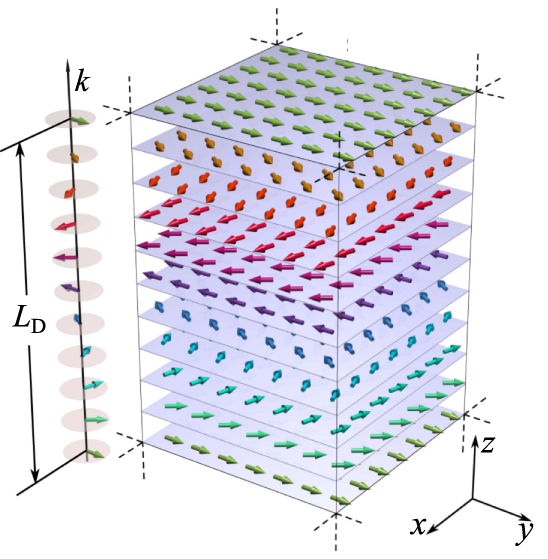
\includegraphics[width=\textwidth]{Figures/helicalspiral.png}
   \caption{}
   \label{fig:mnge_spiral}
\end{subfigure}
\begin{subfigure}[b]{0.49\textwidth}
	\includegraphics[width=\textwidth]{Figures/B20_hedgehog_antihedgehog.pdf}
   \caption{}
   \label{fig:mnge_3q}
\end{subfigure}
	\caption{Magnetic textures that are found experimentally in B20-\ce{MnGe}:  (a) Helical
	spin spiral that propagates in (001) direction. Figure is raken from \cite{rybakov_new_2016} b) 
	Magnetic anti-hedgehog texture that is wrapped around a magnetic monopole at the center. Figure is taken from \cite{zhang_electric_2016}.}
\label{fig:mnge_spiral_and_3q}
\end{figure}



Lately, special attention has been paid to cubic B20-type compounds with broken lattice inversion symmetry,
where skyrmion phases have been observed experimentally \cite{nagaosa_topological_2013}.
In a recent study \cite{tanigaki_real-space_2015} it was 
found by real-space observation transmission electron microscopy that a cubic lattice of skyrmionic hedgehogs
and anti-hedgehogs (see \Cref{fig:mnge_3q}) exists in B20-\ce{MnGe} 
with a lattice constant of about 3-6 nm.
Findings by Kanazawa et al. suggest that this lattice is set up by a superposition of three orthogonal
helical structures also referred to as 3Q state \cite{kanazawa_noncentrosymmetric_2017}. 
While the 3Q state certainly constitutes the most interesting non-trivial magnetic texture 
in B20-\ce{MnGe} there are also reports that the magnetic ground state in this system is
actually a helical spiral (see \Cref{fig:mnge_spiral}) \cite{yaouanc_magnetic_2017}.
These two observations are clearly contradictory and it was not yet explained how
both can be made within the same material.

Therefore, we performed
an analysis of these two helical states and the trivial ferromagnetic (FM) state.
The ferromagnet was identified as the ground state in the small unit cell (8 atoms), 
in which 1Q and 3Q state with their wavelengths of
3-6 nm do not fit.
\\
We begin by setting up a 6x6x6 B20-\ce{MnGe} supercell (1728 atoms), where we use PBEsol 
as exchange-correlation functional
and include only a single k-point, i.e. the $\gamma$-point.
In this initial comparison of ferromagnetic, 1Q and 3Q state using the equilibrium lattice constant
$a=4.80$ \AA \, the ferromagnet is predicted to be the ground state.
As this contradicts experimental observations we take into consideration that
in experiment the crystal structure might inadvertently differ from the ideal structure.
Such discrepancies can be caused e.g. by strain.
\\
Therefore, it is reasonable to check whether a material's properties change, when the
lattice constant is varied.
\begin{figure}[h]
\begin{center}
 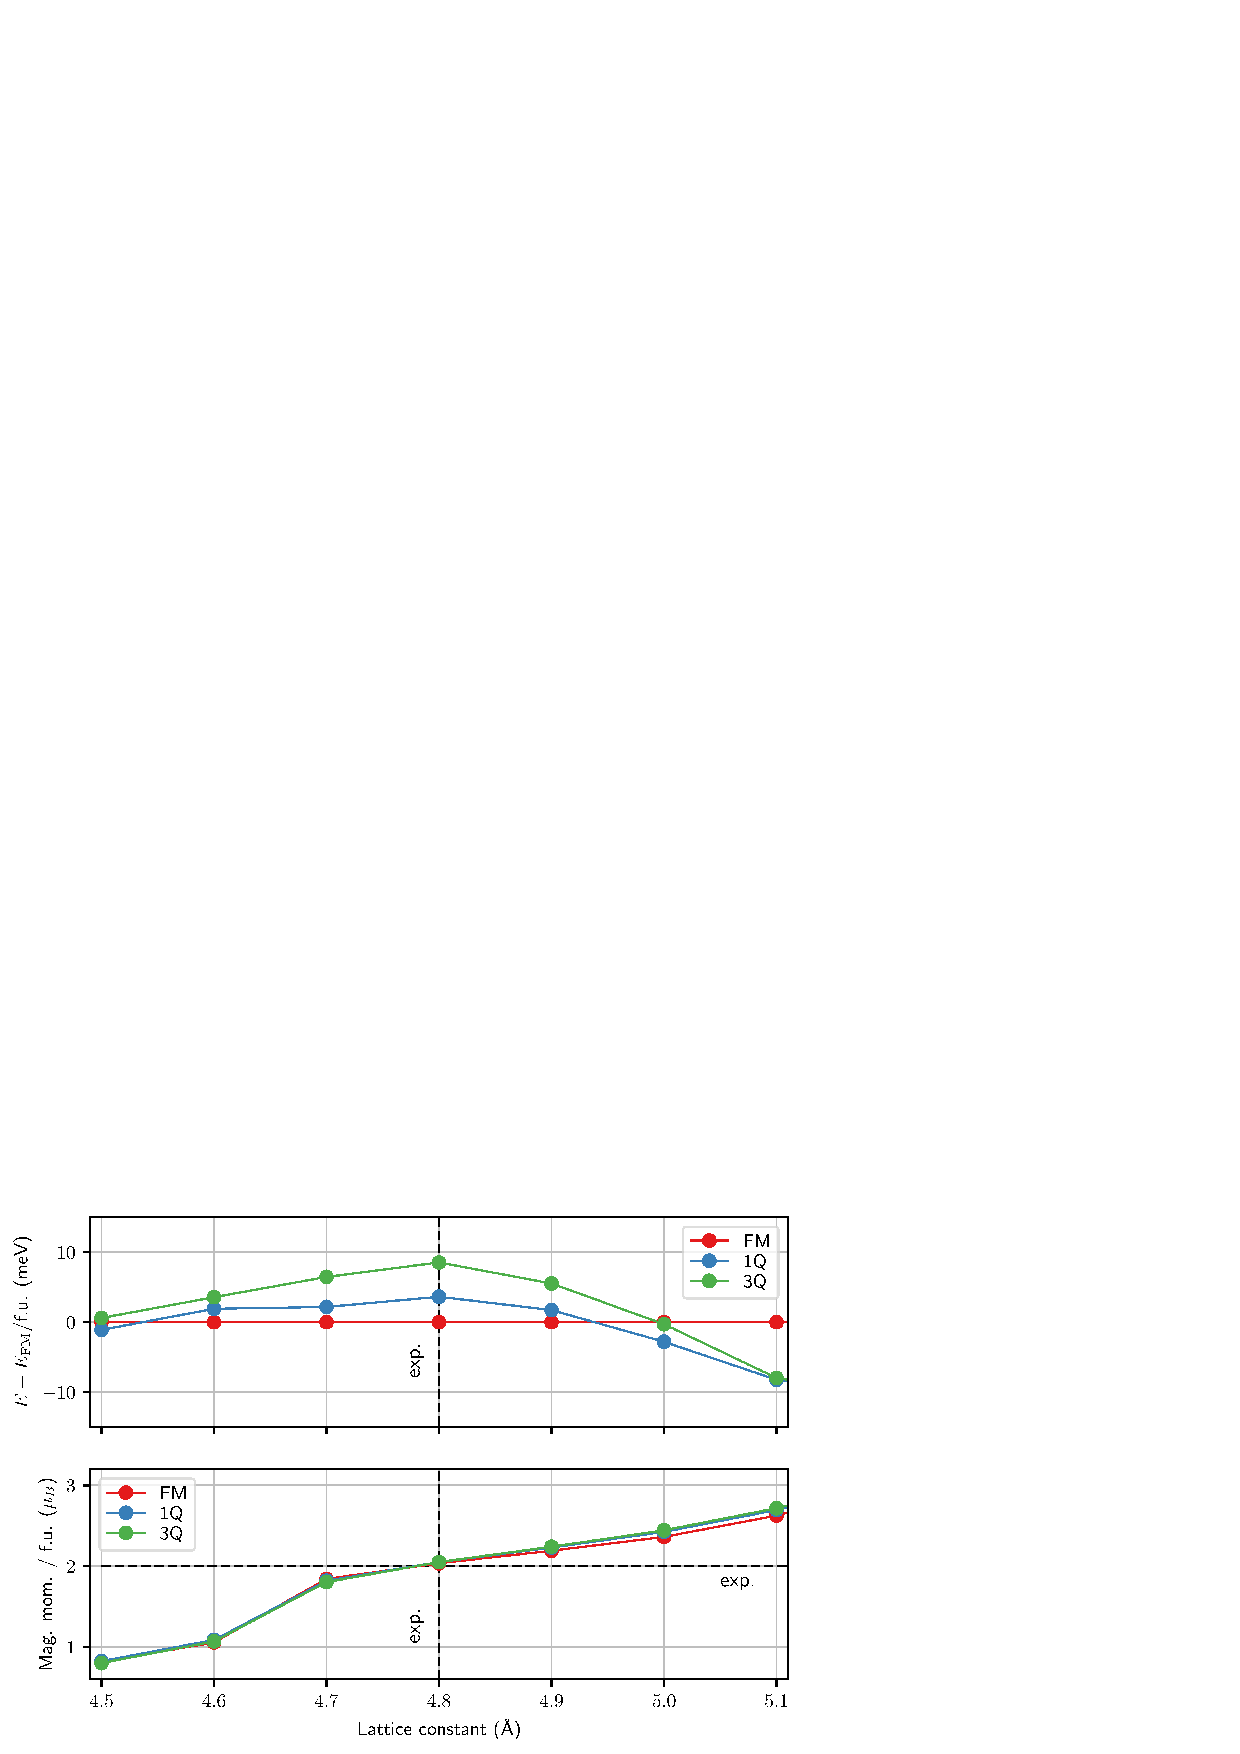
\includegraphics[width=\textwidth]{Figures/MnGe_ferro_1q.pdf}
\end{center}
\caption{
	Comparison of Ferromagnetic (FM), helical spiral (1Q) and hedgehog lattice (3Q) state with KKRnano.
	Top: Difference of total energies with the FM state as reference state for different lattice constants. 
	The experimental lattice constant is a = 4.80 \AA. 1Q and 3Q state are energetically preferrable 
	for $a > 5.0$ \AA. Bottom: Magnetic moment per Mn atom increases with lattice constant. 
	High-spin/Low-spin transition is clearly visible between a = 4.60 and a = 4.70 \AA.
	Experimentally, the magnetic moment is measured to be $\approx 2 \mu_{B}$.
	}
\label{fig:MnGe_ferro_1q}
\end{figure}
Such a variation is performed in the upper part of \Cref{fig:MnGe_ferro_1q}, where
the total energy is evaluated for FM, 1Q and 3Q state.
Clearly, neither the 1Q nor the 3Q state constitutes the ground state,
when the experimental lattice constant is assumed.
Yet, by increasing or decreasing the lattice constant the energetic difference can be made
smaller.
\\
We focus on an increase of the lattice constant rather than a decrease since 
the system goes into the low-spin state below $a=4.65$ \AA \, and according to experiment
the non-trivial textures
exist in the high-spin regime.
A crucial transition point is found around $a=5.0$ \AA,
where by imposing the 1Q or 3Q state the energy can be made smaller than for the ferromagnetic state.
In general, for $a>5.0$ \AA both helical states are favored over the ferromagnet.
\\
Obviously, an artifical increase of the lattice constant by
$0.2$ \AA \, ($\approx 4 \%$) or more is fairly large.
However, probes in experiment are seldom if ever perfectly clean and
impurities in the sample need to be considered as a source of error in the
final analysis. One potential
effect of impurities is chemical pressure that causes a spatial expansion of the
lattice structure.
An example of the possible effects of positive chemical pressure
can be found in \ce{Co}-doped B20-\ce{FeGe} \cite{stolt_chemical_2018}. 
Here, it was experimentally observed
that doping can increase the melting temperature and magnetic properties of a B20 alloy.
\\
In the lower part of \Cref{fig:MnGe_ferro_1q} the evolution of the magnetic moment
with decreasing/increasing lattice constant is tracked.
The resulting magnetic moment for the experimental lattice constant nicely falls 
on top of the magnetic moment of approximately $2 \mu_{B}$/f.u. 
which is reported by experimentalists \cite{yaouanc_magnetic_2017}.
\\
The high-spin/low-spin transition is recognizable between $a=4.60$ and $a=4.70$ \AA.
\\
Furhtermore, the magnetic moment increases, when the lattice constant is increased.
This is a common behaviour in DFT for metallic systems.
For larger lattice constants the magnetic moments of the three different
magnetic textures differ more than for the smaller lattice constants.
This could also give rise to the differences in the total energy.



\newpage

\bibliography{My_Library}

%\section{Bibliographic References}
%\rule{\textwidth}{0.4pt}\\
%\textit{Provide recent/most important bibliographic references that are relevant to the project.}\\

\bigskip
\begin{flushright}
{\tiny V1.3-2016JUN07}
\end{flushright}
\end{document}
